In this chapter the implementation of the server-side of the system is described. \todo{Kilder hvor relevant}

\section{Choice of Server Hosting}
Two different options were investigated with regards to the hosting of the web-service. The first option researched was to host the system on a web server. This could either be done as a dedicated or virtual server. The second option was to host it on a cloud computing platform.

It was considered to set up a virtual machine to host the web service, as it is the traditional way to do things, and it would most likely have been sufficient for this project. It would have allowed for the web server, API and database to be hosted in one place. However, this solution would not be very scalable, as the system would be limited by a physical or virtual server. More virtual machines could be started, but would still run independent of each other, and doing so would also require another system to host the database for it to be accessible to all machines.

The alternative option was to use a cloud hosting solution. Cloud hosting solutions offers compute services, which is code that can be run in the cloud while being serverless. This would allow our code to scale wide, as it would not be dependent on the underlying server, or other running code, and a theoretically infinite number instances could be run in parallel. Other resources such as databases would be hosted independently, and could then be accessed by using various endpoints.

In this project, it was chosen to use a serverless, cloud hosting solution, because of the high flexibility and scaleablity that this allows. Further more, it allows for less time spent setting up a server and the different solutions needed for a project like this, than by using a classic web server.

A large variety of cloud hosting solutions exist. Some of the major ones are: Amazon AWS, Google Cloud, and Microsoft Azure. To ease the implementation of the personal assistant, Amazon Alexa, it has been decided to use Amazon AWS to host the web service.

\section{AWS}
\label{sec:aws}
Amazon AWS contains several different services and solutions that can be used to implement the server. In this section the different AWS services that is used in the implementation of the web service are explained.

\subsection{ARN}
ARN is short for Amazon Resource Name, and is a way to identify a resource on AWS. The ARN is unique across all AWS services and users. The structure of an ARN varies depending on the service but usually follows the structure \texttt{arn:partition:service:region:account-it:resource}. All ARNs start with \texttt{arn}, followed by a \texttt{partition}, which for most cases is \texttt{aws}. The \texttt{service} is the AWS service it belongs to. This can be \texttt{s3}, \texttt{iam}, \texttt{rds} or any other service. \texttt{region} is the region where the resource is located. For some AWS services, the resource is only made available in specified regions. The \texttt{account-id} is the id of the AWS the resource belongs to. The \texttt{resource} can have different forms depending on what service it belongs to. Not all services makes use of all parts since, as a service such as \texttt{IAM} is region independant. 

\subsection{Lambda}
Lambda functions are pieces of code that can be called from another AWS service, or directly over the internet. They can be programmed using Java, C\#, Python, and Node.js. Since there is no real server for the script to run on, there also is not any system to handle dependencies, so they have to be uploaded together with the script for each Lambda, or alternatively added to S3. The purpose of S3 is further explained in section \ref{s3}.

It is possible to control the Lambdas, limit how much RAM a Lambda can use, and how long they can run before they should timeout, limited to a maximum of 1.5GB of memory, and a running time of 5 minutes. Security policies can also restrict the lambdas such that that they can only interact with other specific AWS services if they have been allowed to do so.

Lambdas is testable directly through Amazons services, as it is possible to create test data from the editor, and run the lambda function on that test data. Each test needs to be run manually. This is another benefit that was taken into consideration when choosing how to host this project.

\subsection{EC2}
To prevent parts of the system from being accessed from the outside it is run through a VPC (Virtual Private Cloud) so that only other systems that are part of the same VPC can interact together. Anything running inside the VPC cannot call services or resources located outside the VPC.

\subsection{RDS}
RDS is shorthand for "Relational Database Service", and can be used to create instances of databases. It is possible to host most common database types, including PostgreSQL, which has been chosen to use in this project. It is also possible to specify how powerful the database is, as well as how big it should be. This allows for the scaling wanted in this project.

RDS uses EC2 security groups to control who can access databases. This means that every connection to the RDS has a specific rule - otherwise no connection is allowed. If for example access to the RDS was required from a personal computer, the specific IP address would have to be whitelisted.


\subsection{API Gateway}
The API Gateway was used to create a REST API. Using API Gateway, it is possible to specify which resources the API should have, as well as what methods each resource has access to. It is possible to interact with many of the AWS systems through the API. The API Gateway also allows restriction of the API, so that API keys are required, or only specific users use the method.

\subsection{IAM}
IAM is a tool for administrating permissions for AWS services for developers. The tool is meant to control what actions different AWS services are allowed to perform, to prevent services from access other services. In this project it was mainly used to allow multiple users to interact with the same AWS service, using different developer accounts.\todo{uddybe mabe?}


\subsection{SNS}
SNS stands for Simple Notification Service, and is a tool that provides functionality for sending messages such as SMS, Email and App notifications. For app notifications AWS does not support iOS and Android directly, so Google Cloud Messaging or Apple Developer also needs to be set up.\todo{måske uddyb at sns sender ud til firebase kris syntes ikke det er tydeligt}

\subsection{S3} \label{s3}
S3 stands for Simple Storage Service and is meant for storing and retrieving data. Use cases include: storing files for sharing, scripts for use with AWS Lambda Functions, and HTML, CSS and JavaScript files for static websites. S3 is the recommended way to host a website, such as the one needed for the control panel. %https://aws.amazon.com/websites/

Websites hosted with S3 are also scalable, as the server can provide the files to more people as demand increases.

\subsection{Communication Between Services}
All of the AWS services work together to form the fall detection service.

\begin{figure}[H]
    \centering
    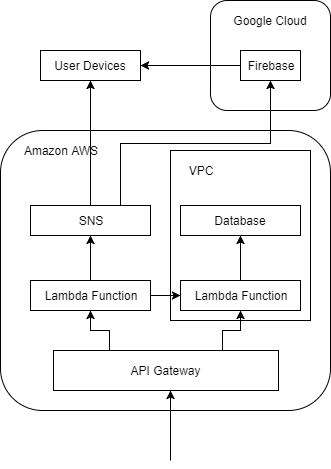
\includegraphics{Figures/aws_diagram.png}
    \caption{Flow of AWS Services}
    \label{fig:aws_diagram}
\end{figure}

Figure \ref{fig:aws_diagram} shows how the order in which the different services are called. All requests from the control panel and devices goes through the API Gateway. The API Gateway then forwards the request data to the connected AWS Lambda Function. The AWS Lambda Function can either run inside or outside a VPC. In this case however, VPC is necessary because it protects the database from outside access. Furthermore, it prevents the AWS Lambda Functions inside the VPC from interacting with the outside world, including sending messages, and starting other lambdas\todo{vpc forklaring måske}.

The AWS Lambda Functions inside the VPC can access the database, perform writing or reading, and return the related objects.

\todo{Forklar at SNS ikke kan tilgås inde i VPCen}
The AWS Lambda Function can also call AWS SNS where it can send notifications and SMS messages. For notifications to Android devices it needs to call Firebase from Google Cloud. The messages are then sent out to the users devices as needed.


\section{Model}\label{model}
In this section the model used to represent elements on the server is explained.

The model was made to make working on data easier and consistent on the server side, and to ensure the presence of important fields in the data types. Three different models are used, where two of them have specialized sub-models.

\subsection{User}
User is a collection of models that describe the different types of users in the system.

The users in the system are:
\begin{itemize}
    \item User: (id, name, email, role) \newline
    The user is the base model for the users in the system. It is used as a middle step for parsing one of the other user types, as the system is unable to properly de-serialize into an inherited type.\todo{what? does this need explanation?}
    \item Citizen: (id, name, email, role, [Contacts], [Device], address, city, postnr) \newline
    The Citizen model describes the citizen.  
    \item Contact: (id, name, email, role, [Devices]) \newline
    The Contact model describes the Contact and its devices.
    \item CitizenAdmin: (id, name, email, role, [Citizens]) \newline
    The model for the user that administrates citizens.
    \item UserAdmin: (id, name, email, role) \newline
    The model for the user that can administrate everything.
\end{itemize}


\subsection{Device}
Device is a collection of models that describe the different devices that the user can use, and the contents of them.

The devices currently supported in the system are:
\begin{itemize}
    \item Device: (id, devicetype)
    The base device, only used for certain error types, and and as a middle step for parsing one of the other types, as the system is unable to properly deserialize into an inherited type.
    \item AppDevice: (id, devicetype, token, arn)
    The AppDevice is the users smartphone. This device is automatically created when the user logs in. It contains the token that is used by SNS and Google Firebase to send notifications to the smartphone.
    \item AlexaDevice: (id, devicetype, user\_id) 
    The AlexaDevice is used to represent an Alexa connected to the user. The Alexa device contains the user identifer related to it, and is used for determining what user it should start an alarm for.
    \item (IFTTTDevice (id, devicetype, token)
    The IFTTTDevice is a device that contains a token for a users IFTTT connected device. When the user has fallen, the token can be used to activate certain devices in the users home.
    \item SmsDevice: (id, devicetype, phone\_number) 
    The SmsDevice is a device that represents a phone device that the system should send an SMS to in the case that a citizen has fallen.
    \item PhoneCallDevice: (id, devicetype, phone\_numboer)
    The same as SmsDevice, but with the intent of calling contacts instead of sending an SMS.
\end{itemize}

The reason SmsDevice and PhoneCallDevice are separate devices, is that the contact should be able to control if they want a SMS or call when getting notified.

\subsection{Alarm}
The Alarm model represents an ongoing alarm that a Citizen has activated. The Alarm has the form (status, citizen, contact). The status is an integer that represents how many contacts that have answered to the alarm, regardless if they can help or not. The citizen is the model of the citizen that has started the alarm. The Contact is the model of a contact that has said that it can help the citizen, if answering using the app. Until then, the Contact space is empty.


\section{API}
In this section the API and underlying implementation is described. First the API itself is presented followed by descriptions of the functionality behind each endpoint.

\begin{figure}[H]
    \centering
    \begin{tabular}{|l|p{2cm}|p{2cm}|p{2cm}|p{2cm}|} \hline
         Resource & GET & POST & PUT & DELETE \\ \hline
         /Citizen/\{id\} & In: \newline - Citizen\_id \newline Out:  \newline - Citizen & \cellcolor{gray!40} & \cellcolor{gray!40} & \cellcolor{gray!40} \\ \hline
         /Contact/\{id\} & In: \newline - Contact\_id \newline Out: \newline - Contact & \cellcolor{gray!40} & \cellcolor{gray!40} & \cellcolor{gray!40} \\ \hline
         /Contact/ & In: \newline - \newline Out:  \newline - [Contact] & \cellcolor{gray!40} & \cellcolor{gray!40} & \cellcolor{gray!40} \\ \hline
         /Citizen/\{id\}/Alarm & In: \newline - Citizen\_id \newline Out: \newline - Alarm & In: \newline - Citizen\_id \newline Out: \newline - Alarm & In: \newline - Alarm \newline Out: \newline - Alarm & In: \newline - Alarm \newline Out: \newline - Alarm \\ \hline
         /.../\{id\}/Device & \cellcolor{gray!40} & In: \newline - Device \newline - User\_id \newline Out: \newline - Device & In: \newline - Device \newline Out: \newline - Device & In: \newline - Device \newline Out: \newline - Device \\ \hline
         /User & In: \newline - email \newline - password \newline Out: \newline - User & In: \newline - User \newline Out: \newline - User & In: \newline - User \newline Out: \newline - User & In: \newline - User \newline Out: \newline - User \\ \hline
    \end{tabular}
    \caption{Api calls}
    \label{table:api}
\end{figure}

The resources on table \ref{table:api} uses the abbreviations Ci\_id, Ca\_id, and Us\_id for ids where the id is given as part of the URL path.

When the API states that it returns Citizens, Contacts, Users, Devices, or Alarms it refers to the full serialized models described in \ref{model}. Even when dealing with errors or representing deleted content, the models are used, just with empty fields and negative id.

\subsection*{Mapping} \label{api:mapping}


\subsection*{Structure}
All AWS Lambda Functions follow the same general structure to make input and output with the API simple and consistent.
All input happens through the event, which is a (string,string) dictionary with the input mapped in \ref{api:mapping}.
It returns an HTML request response with a status code, body and headers.

\begin{figure}[H]
    \centering
    \begin{lstlisting}[language=Python]
        def lambda_handler(event, context)
            try:
                input_var1 = event["input_var1"]
                ...
                
                if not input_var1:
                    # Return error since we have unassigned variables
                    
                # LOGIC
                
                return respond(statuscode, serializedobject)
            except:
                return respond(statuscode, errorobject)
    \end{lstlisting}
    \caption{The base structure of a lambda function}
    \label{fig:samplelambdafunction}
\end{figure}

On figure \ref{fig:samplelambdafunction} it can be seen that it takes event and context as input. Context is never used, but contains information about the AWS Lambda Function itself.
First all arguments are retrieved from event, and assigned. Sometimes they are also deserialized if a model object is expected. Afterwards some error handling is done, before the main logic of the lambda is done.
Response is built from a status code, and the object that it should return. The AWS Lambda Functions does always return an object as shown on figure \ref{table:api}

When returning an error, an object is constructed that follow the same pattern as the otherwise correct object, but with a negative ID, and most other fields as empty strings or arrays, since the error doesn't contain any info.

\subsection*{/User}
The user resource is used for creating and editing users. Making a GET request works as a login, as it unlike all other requests doesn't use the model for requests.

\subsubsection*{Password security}
When a user has created an account they have also provided a password. To keep the passwords secure, they were salted and hashed, so that only the salt and hashed version of the password were saved in the database.

\begin{figure}[H]
    \centering
    \begin{lstlisting}[language=Python]
    def get_salt():
        return uuid.uuid4().hex


    def hash_password(password, salt):
        return hashlib.sha512((password + salt).encode('utf-8')).hexdigest()
    \end{lstlisting}
    \caption{Functions for getting salt and hash password}
    \label{fig:passwordhashing}
\end{figure}

All salt have been generated by using Pythons built-in uuid library\cite{Python:UUID}. The library recommends uuid4 for a random UUID, and the function returns a string of 32 hexadecimal digits. The salt were used to ensure that even if two users have had the same password, it would be stored as different hashed passwords in the database.

When the user have been created, the password is run though a hashing function seen on \ref{fig:passwordhashing} with the salt, and the same function is used again when the user tries to login. On a login the password the user have tried to login with have been hashed with the same salt, and the two hashed passwords are compared. If the hashed passwords are identical the user would be returned. Otherwise an fault user would be returned.


\subsection*{/Citizen/\{id\}}
When an useradmin or citizenadmin needs to request individual users, it is done by adding the citizens id as part of the request.

\subsection*{/Contact/\{id\}}
Like with the citizen, a specific contact is requested by adding the contacts id as part of the request.

\subsection*{/Contact}
When administrating a citizen with the control panel it is necessary to find contacts in the system. This endpoint returns all contacts in the system and is used when the Control Panel needs to search among contacts.

\subsection*{/Citizen/\{id\}/Alarm}
When a citizen have raised an alarm, an alarm object is created. Because the alarm also needs to send out notifications and SMS messages to all contacts related to the citizen, an alarm is created. 

When creating an alarm the alarm AWS Lambda Function also needs to call a second AWS Lambda Function. This is because the alarm both needs to be saved and send notifications, and both cannot happen on the same AWS Lambda Function because the database is running on an VPC.

\begin{figure}[H]
    \centering
    \begin{lstlisting}[language=Python]
    lambda_client = boto3.client('lambda',
        region_name=region_name,
        aws_access_key_id=aws_access_key_id,
        aws_secret_access_key=aws_secret_access_key)

    arg = bytes(json.dumps({"id": ctz_id}), 'utf-8')
    response = lambda_client.invoke(
        FunctionName=arn_alarm_create_endpoint,
        InvocationType="RequestResponse",
        Payload=arg)

    data = response["Payload"].read().decode()
    \end{lstlisting}
    \caption{Code for starting a lambda function from within another lambda function}
    \label{fig:startlambda}
\end{figure}

Because of that the AWS Lambda Function instead calls another AWS Lambda Function using the boto3 library as seen on figure \ref{fig:startlambda}. The new AWS Lambda Function can then create the alarm and store it in the database, before returning it to the calling lambda.

This is necessary because the database runs on an VPC for security reasons. Most AWS Lambda Functions run directly on the VPC since they only need to access the database. When creating an alarm the AWS Lambda Function also needs to access AWS SNS, which isn't reachable from within the VPC, so the work has to be split.

\begin{figure}[H]
    \centering
    \begin{lstlisting}[language=Python]
    def push_message(endpoint_arn, message):
        sns_client = boto3.client(
            'sns',
            region_name=region_name,
            aws_access_key_id=aws_access_key_id,
            aws_secret_access_key=aws_secret_access_key
        )
    
        return sns_client.publish(
            TargetArn=endpoint_arn,
            MessageStructure='string',
            Message=message
        )
    \end{lstlisting}
    \caption{Sending a notification to a device using SNS}
    \label{fig:sns_notification}
\end{figure}

When sending notifications out to devices, it is necessary to have a means to identify what device to send to. As seen on figure \ref{fig:aws_diagram} SNS needs to send the notification via Firebase, which uses device tokens to identify which device it should send to. But since AWS uses ARN endpoints to identify all resources, each token also needs an ARN to identify them. Eash Target ARN for notifications is part of an Application ARN, that is specific for each device, where an Application ARN targets a specific backend such as Firebase for Android notifications.

As seen on figure \ref{fig:sns_notification} when sesing a message, only the ARN for the token is needed. While the Application ARN is needed when adding the token, the tokens ARN can be used directly afterwards when sending an notification, or updating the token in case it has changed.

\begin{figure}[H]
    \centering
    \begin{lstlisting}[language=Python]
        for c in alm.activatedby.contacts:
            for d in c.devices:
                if d.devicetype == "appdevice":
                    if not d.arn or not d.token:
                        continue
                    try:
                        push_message(d.arn, alm.serialize())
                    except:
                        print("ARN NOT ACTIVE: " + d.arn)
                elif d.devicetype == "smsdevice":
                    send_sms(d.phone_number, c.activatedby.name + " has had an falling accident, and requests help.")

        for d in alm.activatedby.devices:
            if d.devicetype == "iftttdevice":
                urllib.request.urlopen(
                    "https://maker.ifttt.com/trigger/fall_detected/with/key/" + d.token).read()
    \end{lstlisting}
    \caption{Sending notifications out to all contacts, and triggering all IFTTT hooks}
    \label{fig:notify_contacts}
\end{figure}

On figure \ref{fig:notify_contacts} is the code for sending notifications after a citizen has had a falling accident. The code makes sure that all contacts related to the citizen are notifies by SMS and notification. For notifications it needs to make sure that the endpoint exist, and in the case that the endpoint cannot be reached because it is not active, it should log it. When sending an SMS it is important that the provided number also has the correct country code, as SNS can send SMS messages to the entire world, and wouldn't know where to send it otherwise.



\subsection*{/.../\{id\}/Device}
This resource is used by both Citizen and Contact to create and update devices. While the device resource is the same for both citizens and contacts, it was added to both of them to make the API easier to use.

Devices such as Alexa, And a smartphone for calling/sending an SMS is set up using the Control Panel. AppDevice is automatically added and removed from the system as users log in and out. 

The AlexaDevice is used by the citizen to raise an Alarm when the citizen talks to it, but this device can due to technical limitations not be used to send messages back to the citizen, or establish direct communication between the citizen and contact.

The IFTTTDevices are activated when the citizen has has a falling accident, as a message is sent to the IFTTT webhook for the device.

SmsDevice and PhoneCallDevice are both phone devices that contains a phone number. They are differentiated to make it clear to the system whether they should send and SMS or make a call when a citizen has had a falling accident.

The AppDevice currently adds itself to the device list of the user when they have logged in, while it removes itself when they have logged out. The AppDevice is a device that the system can send an notification to when a citizen has had a falling accident.
As explained in \ref{chapter:app} the contact gets the notification after the citizen has fallen, and can say if they can help or not. Either way, when they answer they send the alarm included with the notification back to the server. If they can help, the app includes the contact as a responder, and notifies the citizen by notification that help is on the way, and who is going to help.

\subsection*{Authentication}

To ensure that users only access the parts of the API that they are allowed to, an authentication layer has been added. When a user logs in, they are given an authentication token. This token needs to be provided together with any request made to the rest of the API to ensure that they only have access to the things that they need. It also prevents unauthorized people from doing malicious things. Table \ref{table:auth} shows which resources and methods each user can access. A user is assigned a token when they log in to the system through the API.


% Please add the following required packages to your document preamble:
% \usepackage[table,xcdraw]{xcolor}
% If you use beamer only pass "xcolor=table" option, i.e. \documentclass[xcolor=table]{beamer}
\begin{table}[H]
\centering

\begin{tabular}{|l|l|l|l|l|l|}
\hline
                    & Citizen                                                     & Contact                                                     & User admin                                                  & Citizen admin            & No auth                                        \\ \hline
/citizen/id/        & GET                                                         & \cellcolor[HTML]{9B9B9B}{\color[HTML]{9B9B9B} }             & GET                                                         & GET                      & \cellcolor[HTML]{9B9B9B}                                 \\ \hline
/contact/id/        & \cellcolor[HTML]{9B9B9B}                                    & \cellcolor[HTML]{9B9B9B}{\color[HTML]{9B9B9B} }             & \cellcolor[HTML]{9B9B9B}                                    & \cellcolor[HTML]{9B9B9B} & \cellcolor[HTML]{9B9B9B}                                 \\ \hline
/contact/           & GET                                                         & GET                                                         & GET                                                         & GET                      & \cellcolor[HTML]{9B9B9B}                                 \\ \hline
/citizen/id/alarm/  & POST                                                        & \begin{tabular}[c]{@{}l@{}}GET\\ POST\end{tabular}          & \cellcolor[HTML]{9B9B9B}                                    & \cellcolor[HTML]{9B9B9B} & \cellcolor[HTML]{9B9B9B}                                 \\ \hline
/citizen/id/device/ & \begin{tabular}[c]{@{}l@{}}POST\\ PUT\\ DELETE\end{tabular} & \cellcolor[HTML]{9B9B9B}                                    & \begin{tabular}[c]{@{}l@{}}POST\\ PUT\\ DELETE\end{tabular} & \cellcolor[HTML]{9B9B9B} & \cellcolor[HTML]{9B9B9B}                                 \\ \hline
/contact/id/device/ & \cellcolor[HTML]{9B9B9B}                                    & \begin{tabular}[c]{@{}l@{}}POST\\ PUT\\ DELETE\end{tabular} & \begin{tabular}[c]{@{}l@{}}POST\\ PUT\\ DELETE\end{tabular} & \cellcolor[HTML]{9B9B9B} & \cellcolor[HTML]{9B9B9B}                                 \\ \hline
/user/              & \cellcolor[HTML]{9B9B9B}                                    & \cellcolor[HTML]{9B9B9B}                                    & \cellcolor[HTML]{9B9B9B}                                    & \cellcolor[HTML]{9B9B9B} & \begin{tabular}[c]{@{}l@{}}GET\\ POST\\ PUT\end{tabular} \\ \hline
\end{tabular}
\caption{Table of user authorizations}
\label{table:auth}
\end{table}

The AWS API Gateway includes a tool to add authorizers to an API. This is done by defining an AWS lambda function to handle the authorization request, which returns an IAM, explained in section \ref{sec:aws}. The authorizer takes an authentication token as a parameter, the source of which must be defined when setting up the authorizer, in this case, the source is a header called \textit{token}.

The token is generated using the JSON Web Tokens (JWT) standard \cite{JWT}. Due to the compact size of a JWT, this makes it possible to send it through the request header. Further more, it is self-contained, meaning that the token contains all required information, which means that a call to the database is not required during the authorization step. Each token is signed using a secret string.

\begin{figure}[H]
    \centering
    \begin{lstlisting}[language=Python]
    Header:
    {
        "typ": "JWT",
        "alg": "HS256"
    }
    
    Payload:
    {
        "user_id": "234",
        "user_role": "citizen"
    }
    
\end{lstlisting}
    \caption{Decoded JSON Web Tokens}
    \label{fig:jwt-decoded}
\end{figure}

A JWT consists of three parts, namely the header, payload and signature. An example of a JWT, used in the API test, can be found on table \ref{fig:jwt-decoded}. The header contains information about the type if the token, which is \textit{JWT}, and the hashing algorithm used, in this case \textit{HS256}. The payload contains the data that the token contains. In this example it contains a user id and user role, used by the authorizer to create the IAM. The third part, which is not shown in the example, is the signature part. This part contains information needed to verify the token, including the secret string needed to verify the token.

The three parts of the JWT is encoded and separated by a period  ('.'). The encoded version of the example on figure \ref{fig:jwt-decoded} can be found on figure \ref{fig:jwt-encoded}.

\begin{figure}[H]
    \centering
    \begin{lstlisting}[language=Python]
    eyJ0eXAiOiJKV1QiLCJhbGciOiJIUzI1NiJ9.
    eyJ1c2VyX2lkIjoiMjM0IiwidXNlcl9yb2xlIjoiY2l0aXplbiJ9.
    Lk0L4BX6Dx0b6PlfWMlSp3xFv5o7lYmya2PyAc-FQdE
\end{lstlisting}
    \caption{Encoded JSON Web Tokens}
    \label{fig:jwt-encoded}
\end{figure}

A template, supplied by Amazon, is used to generate the IAM for the authorization request, and a Python library called PyJWT is used to handle the JWT and validation of these. How this is used is demonstrated on figure \ref{fig:iam-auth}.


\begin{figure}[H]
    \centering
    \begin{lstlisting}[language=Python]
    token = jwt.decode(event["authorizationToken"], "power123")
    arn = event["methodArn"]
    
    principalId = token["user_id"]

    tmp = event['methodArn'].split(':')
    apiGatewayArnTmp = tmp[5].split('/')
    awsAccountId = tmp[4]

    policy = AuthPolicy(principalId, awsAccountId)
    policy.restApiId = apiGatewayArnTmp[0]
    policy.region = tmp[3]
    policy.stage = apiGatewayArnTmp[1]
    
    if token["user_role"] == "citizen":
        policy.allowMethod(HttpVerb.POST, '/citizen/*/alarm')
        policy.allowMethod(HttpVerb.ALL, '/citizen/*/device')
        policy.allowMethod(HttpVerb.GET, '/citizen/*')
        
    elif token["user_role"] == "contact":
        policy.allowMethod(HttpVerb.ALL, '/contact/*/device')
        policy.allowMethod(HttpVerb.PUT, '/citizen/*/alarm')
        
    elif token["user_role"] == "citizenAdmin":
        policy.allowMethod(HttpVerb.ALL, '/citizen/*/device')
        policy.allowMethod(HttpVerb.GET, '/citizen/*')
        
    elif token["user_role"] == "userAdmin":
        policy.allowAllMethods()
        policy.allowMethod(HttpVerb.ALL, '/citizen/*/alarm')
    
    
    authResponse = policy.build()
 

    return authResponse
    
    
\end{lstlisting}
    \caption{Snippet from \textit{ProjectFallAuthenticator}}
    \label{fig:iam-auth}
\end{figure}

The authorization lambda is passed two values through its header by the API, namely the \textit{authorizationToken} and \textit{methodArn}. The first of which is the token passed by the caller and the second is the \textit{arn} of the method that the user tried to access. \todo{forklar arn}

The first thing that happens during the authentication process, is that the passed token is decoded. This is done using the PyJWT library. During the decoding of the token, it is also validated using a supplied secret string. In this example the string is \textit{'power123'}. The valuation can be seen on line 1 of the example code. On lines 15 through 30, the allowed methods are added to the IAM, depending on the user type contained in the token. Lastly the IAM is build and returned to the API as a response.

%%%%%%%%%%%%%%%%%%%%%%%%%%%%%%%%%%%%%%%%%%%%%%%%%



\section{Database}

\todo{Sammenlign med design}

In this section we will talk about the implementation of the database. PostgreSQL was chosen as DBMS, since AWS RDS supports it, and it is a known dialect of SQL.

The database has 11 tables to describe users, devices, alarms, and their relations. The database manager is a single file that is responsible for all communication with the database, to keep it at one place. To make interaction with the rest of the system simple and consistent, the database manager functions takes model objects or ids as input and output, so that tuples from the database are kept within the individual functions. 

\subsection{Psycopg2}
Psycopg2 is a library that allows python to interact with a PostgreSQL database. Since AWS does not provide this library itself we need to upload the library together with each lambda. A modified version of Psycopg2 compiled specifically for AWS Lambdas have been used.

\begin{figure}[H]
    \centering
    \begin{lstlisting}[language=Python]
    conn = psycopg2.connect(connect_str)
    cursor = conn.cursor()

    cursor.execute("QUERY")
    res = cursor.fetchone()
    conn.commit()
    cursor.close()
    conn.close()
\end{lstlisting}
    \caption{Example of Psycopg2 interacting with a database}
    \label{fig:psycopg2example}
\end{figure}

The code on figure \ref{fig:psycopg2example} shows how the database can be interacted with. A connection is created using a connection string, containing info about the database and credentials. A curser can then be used to execute queries and fetch results. After running the queries they are committed and the database is closed.

